\documentclass[
	% -- opções da classe memoir --
	12pt,				% tamanho da fonte
	openright,			% capítulos começam em pág ímpar (insere página vazia caso preciso)
	twoside,			% para impressão em verso e anverso. Oposto a oneside
	a4paper,			% tamanho do papel. 
	% -- opções da classe abntex2 --
	%chapter=TITLE,		% títulos de capítulos convertidos em letras maiúsculas
	%section=TITLE,		% títulos de seções convertidos em letras maiúsculas
	%subsection=TITLE,	% títulos de subseções convertidos em letras maiúsculas
	%subsubsection=TITLE,% títulos de subsubseções convertidos em letras maiúsculas
	% -- opções do pacote babel --
	english,			% idioma adicional para hifenização
%	french,				% idioma adicional para hifenização
%	spanish,			% idioma adicional para hifenização
	brazil,				% o último idioma é o principal do documento
	]{abntex2}

% O documento abaixo tem que vir antes do \usepackage{tcc} para poder aproveitar os valores
% informados nas macros dentro de capa_e_folhaRosto

\usepackage{tcc}
% ---
% Informações de dados para CAPA e FOLHA DE ROSTO
% ---
\titulo{Comparação de Estratégias Estatísticas para Aferição de Qualidade Visual}
\autor{Luiz Felipe Angioletti Soares}
\local{Belém}
\data{\today}
\orientador{Prof. Dr. Ronaldo de Freitas Zampolo}
%\coorientador{Equipe \abnTeX}
\instituicao{%
  Universidade Federal do Pará -- UFPA
  \par
  Instituto de Tecnologia
  \par
  Faculdade de Engenharia da Computação e Telecomunicações
  \par
  Programa de Graduação em Engenharia da Computação}
\tipotrabalho{Trabalho de Conclusão de Curso}
% O preambulo deve conter o tipo do trabalho, o objetivo, 
% o nome da instituição e a área de concentração 
\preambulo{Trabalho de Conclusão de Curso para obtenção de grau de Engenheiro da 
Computação pela Faculdade de Engenharia da Computação e Telecomunicações,
Instituto de Tecnologia, Universidade Federal do Pará.}
% ---


% ---
% Configurações de aparência do PDF final

% alterando o aspecto da cor azul
\definecolor{blue}{RGB}{41,5,195}

% informações do PDF
\makeatletter
\hypersetup{
     	%pagebackref=true,
		pdftitle={\@title}, 
		pdfauthor={\@author},
    	pdfsubject={\imprimirpreambulo},
	    pdfcreator={LaTeX with abnTeX2},
		pdfkeywords={abnt}{latex}{abntex}{abntex2}{trabalho acadêmico}, 
		colorlinks=true,       		% false: boxed links; true: colored links
    	linkcolor=blue,          	% color of internal links
    	citecolor=blue,        		% color of links to bibliography
    	filecolor=magenta,      		% color of file links
		urlcolor=blue,
		bookmarksdepth=4
}
\makeatother
% --- 

% --- 
% Espaçamentos entre linhas e parágrafos 
% --- 

% O tamanho do parágrafo é dado por:
\setlength{\parindent}{1.3cm}

% Controle do espaçamento entre um parágrafo e outro:
\setlength{\parskip}{0.2cm}  % tente também \onelineskip

% ---
% compila o indice
% ---
\makeindex
% ---



%
%
% DICAS GERAIS:
%	* LEIA O TEXTO ESCRITO
%	* ATIVE OS REVISORES GRAMATICAIS
%	* PREOCUPE-SE INICIALMENTE COM O CONTEÚDO, DEIXE PARA DEPOIS A ESTÉTICA E A EDIÇÃO
%	* SEJA OBJETIVO E EVITE REDUNDÂNCIA
%	* NUMERE AS EQUAÇÕES
%	* PARA AS LISTAS, TENTE USAR AS FUNÇÕES AUTOMÁTICAS DOS EDITORES
%	* IDEM PARA AS REFERÊNCIAS
%
%
\begin{document}
% Retira espaço extra obsoleto entre as frases.
%\frenchspacing 

% ----------------------------------------------------------
% ELEMENTOS PRÉ-TEXTUAIS
% ----------------------------------------------------------
\pretextual

% ---
% Capa
% ---

\imprimircapa
% ---

% ---
% Folha de rosto
% (o * indica que haverá a ficha bibliográfica)
% ---
\imprimirfolhaderosto*
% ---

%% ---
% Inserir a ficha bibliografica
% ---

% Isto é um exemplo de Ficha Catalográfica, ou ``Dados internacionais de
% catalogação-na-publicação''. Você pode utilizar este modelo como referência. 
% Porém, provavelmente a biblioteca da sua universidade lhe fornecerá um PDF
% com a ficha catalográfica definitiva após a defesa do trabalho. Quando estiver
% com o documento, salve-o como PDF no diretório do seu projeto e substitua todo
% o conteúdo de implementação deste arquivo pelo comando abaixo:
%
% \begin{fichacatalografica}
%     \includepdf{fig_ficha_catalografica.pdf}
% \end{fichacatalografica}
\begin{fichacatalografica}
	\vspace*{\fill}					% Posição vertical
	\hrule							% Linha horizontal
	\begin{center}					% Minipage Centralizado
	\begin{minipage}[c]{12.5cm}		% Largura
	
	\imprimirautor
	
	\hspace{0.5cm} \imprimirtitulo  / \imprimirautor. --
	\imprimirlocal, \imprimirdata-
	
	\hspace{0.5cm} \pageref{LastPage} p. : il. (algumas color.) ; 30 cm.\\
	
	\hspace{0.5cm} \imprimirorientadorRotulo~\imprimirorientador\\
	
	\hspace{0.5cm}
	\parbox[t]{\textwidth}{\imprimirtipotrabalho~--~\imprimirinstituicao,
	\imprimirdata.}\\
	
	\hspace{0.5cm}
		1. Palavra-chave1.
		2. Palavra-chave2.
		I. Orientador.
		II. Universidade xxx.
		III. Faculdade de xxx.
		IV. Título\\ 			
	
	\hspace{8.75cm} CDU 02:141:005.7\\
	
	\end{minipage}
	\end{center}
	\hrule
\end{fichacatalografica}
% ---

%% ---
% Inserir errata
% ---
\begin{errata}
Elemento opcional da \citeonline[4.2.1.2]{NBR14724:2011}. Exemplo:

\vspace{\onelineskip}

FERRIGNO, C. R. A. \textbf{Tratamento de neoplasias ósseas apendiculares com
reimplantação de enxerto ósseo autólogo autoclavado associado ao plasma
rico em plaquetas}: estudo crítico na cirurgia de preservação de membro em
cães. 2011. 128 f. Tese (Livre-Docência) - Faculdade de Medicina Veterinária e
Zootecnia, Universidade de São Paulo, São Paulo, 2011.

\begin{table}[htb]
\center
\footnotesize
\begin{tabular}{|p{1.4cm}|p{1cm}|p{3cm}|p{3cm}|}
  \hline
   \textbf{Folha} & \textbf{Linha}  & \textbf{Onde se lê}  & \textbf{Leia-se}  \\
    \hline
    1 & 10 & auto-conclavo & autoconclavo\\
   \hline
\end{tabular}
\end{table}

\end{errata}
% ---

%% ---
% Inserir folha de aprovação
% ---

% Isto é um exemplo de Folha de aprovação, elemento obrigatório da NBR
% 14724/2011 (seção 4.2.1.3). Você pode utilizar este modelo até a aprovação
% do trabalho. Após isso, substitua todo o conteúdo deste arquivo por uma
% imagem da página assinada pela banca com o comando abaixo:
%
% \includepdf{folhadeaprovacao_final.pdf}
%
\begin{folhadeaprovacao}

  \begin{center}
    {\ABNTEXchapterfont\large\imprimirautor}

    \vspace*{\fill}\vspace*{\fill}
    {\ABNTEXchapterfont\bfseries\Large\imprimirtitulo}
    \vspace*{\fill}
    
    \hspace{.45\textwidth}
    \begin{minipage}{.5\textwidth}
        \imprimirpreambulo
    \end{minipage}%
    \vspace*{\fill}
   \end{center}
    
   Trabalho aprovado. \imprimirlocal, 24 de novembro de 2012:

   \assinatura{\textbf{\imprimirorientador} \\ Orientador} 
   \assinatura{\textbf{Professor} \\ Convidado 1}
   \assinatura{\textbf{Professor} \\ Convidado 2}
   %\assinatura{\textbf{Professor} \\ Convidado 3}
   %\assinatura{\textbf{Professor} \\ Convidado 4}
      
   \begin{center}
    \vspace*{0.5cm}
    {\large\imprimirlocal}
    \par
    {\large\imprimirdata}
    \vspace*{1cm}
  \end{center}
  
\end{folhadeaprovacao}
% ---

%% ---
% Dedicatória
% ---
\begin{dedicatoria}
   \vspace*{\fill}
   \centering
   \noindent
   \textit{ Este trabalho é dedicado às crianças adultas que,\\
   quando pequenas, sonharam em se tornar cientistas.} \vspace*{\fill}
\end{dedicatoria}
% ---

%% ---
% Agradecimentos
% ---
\begin{agradecimentos}
Os agradecimentos principais são direcionados à Gerald Weber, Miguel Frasson,
Leslie H. Watter, Bruno Parente Lima, Flávio de Vasconcellos Corrêa, Otavio Real
Salvador, Renato Machnievscz\footnote{Os nomes dos integrantes do primeiro
projeto abn\TeX\ foram extraídos de
\url{http://codigolivre.org.br/projects/abntex/}} e todos aqueles que
contribuíram para que a produção de trabalhos acadêmicos conforme
as normas ABNT com \LaTeX\ fosse possível.

Agradecimentos especiais são direcionados ao Centro de Pesquisa em Arquitetura
da Informação\footnote{\url{http://www.cpai.unb.br/}} da Universidade de
Brasília (CPAI), ao grupo de usuários
\emph{latex-br}\footnote{\url{http://groups.google.com/group/latex-br}} e aos
novos voluntários do grupo
\emph{\abnTeX}\footnote{\url{http://groups.google.com/group/abntex2} e
\url{http://abntex2.googlecode.com/}}~que contribuíram e que ainda
contribuirão para a evolução do \abnTeX.

\end{agradecimentos}
% ---

%% ---
% Epigrafe
% ---
\begin{epigrafe}
    \vspace*{\fill}
	\begin{flushright}
		\textit{``Não vos amoldeis às estruturas deste mundo, \\
		mas transformai-vos pela renovação da mente, \\
		a fim de distinguir qual é a vontade de Deus: \\
		o que é bom, o que Lhe é agradável, o que é perfeito.\\
		(Bíblia Sagrada, Romanos 12, 2)}
	\end{flushright}
\end{epigrafe}
% ---

%% ---
% RESUMOS
% ---

% resumo em português
\begin{resumo}
 Segundo a \citeonline[3.1-3.2]{NBR6028:2003}, o resumo deve ressaltar o
 objetivo, o método, os resultados e as conclusões do documento. A ordem e a extensão
 destes itens dependem do tipo de resumo (informativo ou indicativo) e do
 tratamento que cada item recebe no documento original. O resumo deve ser
 precedido da referência do documento, com exceção do resumo inserido no
 próprio documento. (\ldots) As palavras-chave devem figurar logo abaixo do
 resumo, antecedidas da expressão Palavras-chave:, separadas entre si por
 ponto e finalizadas também por ponto.

 \vspace{\onelineskip}
    
 \noindent
 \textbf{Palavras-chaves}: latex. abntex. editoração de texto.
\end{resumo}

% resumo em inglês
\begin{resumo}[Abstract]
 \begin{otherlanguage*}{english}
   This is the english abstract.

   \vspace{\onelineskip}
 
   \noindent 
   \textbf{Key-words}: latex. abntex. text editoration.
 \end{otherlanguage*}
\end{resumo}

% resumo em francês 
\begin{resumo}[Résumé]
 \begin{otherlanguage*}{french}
    Il s'agit d'un résumé en français.
 
   \vspace{\onelineskip}
 
   \noindent
   \textbf{Mots-clés}: latex. abntex. publication de textes.
 \end{otherlanguage*}
\end{resumo}

% resumo em espanhol
\begin{resumo}[Resumen]
 \begin{otherlanguage*}{spanish}
   Este es el resumen en español.
  
   \vspace{\onelineskip}
 
   \noindent
   \textbf{Palabras clave}: latex. abntex. publicación de textos.
 \end{otherlanguage*}
\end{resumo}
% ---

%% ---
% inserir lista de ilustrações
% ---
\pdfbookmark[0]{\listfigurename}{lof}
\listoffigures*
\cleardoublepage
% ---

%% ---
% inserir lista de tabelas
% ---
\pdfbookmark[0]{\listtablename}{lot}
\listoftables*
\cleardoublepage
% ---

%% ---
% inserir lista de abreviaturas e siglas
% ---
\begin{siglas}
  \item[Fig.] Area of the $i^{th}$ component
  \item[456] Isto é um número
  \item[123] Isto é outro número
  \item[lauro cesar] este é o meu nome
\end{siglas}
% ---

%% ---
% inserir lista de símbolos
% ---
\begin{simbolos}
  \item[$ \Gamma $] Letra grega Gama
  \item[$ \Lambda $] Lambda
  \item[$ \zeta $] Letra grega minúscula zeta
  \item[$ \in $] Pertence
\end{simbolos}
% ---


%% ---
% inserir o sumario
% ---
\pdfbookmark[0]{\contentsname}{toc}
\tableofcontents*
\cleardoublepage
% ---



\textual

% ----------------------------------------------------------
% Introdução
% ----------------------------------------------------------
\chapter{Introdução} \label{chap:intro}

%% Histórico

	Ao longo dos últimos quarenta anos, com a difusão de tecnologias eletrônicas modernas, a palavra ``digital'' tem se tornado cada vez mais lugar comum. Ao longo desse período, a tecnologia baseada em máquinas de cálculo automatizado que ocupavam prédios inteiros e eram operadas por poucos (para fins restritos) foi permeando nossa cultura global e ganhando destaque em vários campos do conhecimento e da vida humanas. Com o passar do tempo, as suas aplicações foram ganhando horizontes, os computadores passaram a ser pessoais e cada vez mais amplamente utilizados, contudo, ainda tinham aplicações específicas em ambientes de pesquisa e para atividades profissionais, e eram restritos a mesas e ambientes reservados. Em paralelo, a indústria de jogos eletrônicos começa a florescer, se fazendo presente nas residências através de seus consoles. Todos aproveitavam a evolução tecnológica apresentada pelo advento dos transistores e microprocessadores.

	Adiante mais alguns anos, e a internet aparece, os microprocessadores estão mais ``micro'' e mais ``processadores'', os consoles de video-game mais elaborados e seus clientes cada vez mais exigentes. Os microprocessadores vão transitando de máquinas estáticas para aplicações móveis: celulares e câmeras digitais (para foto e vídeo) tornam-se quase onipresentes. Mídias digitais tornam-se tão importantes quanto protocolos de comunicação, redes sociais movimentam a opinião pública e servem de plataforma a revoluções ~\cite{revoltaEgito}. Muitos cidadãos globais têm contas em várias redes sociais e máquinas portáteis em seus bolsos, prontas a fazer um vídeo ou uma foto e postá-los para apreciação popular. Ao que se faz possível, com alguns poucos cliques e nenhum custo com passagem ou hospedagem, termos acesso à realidade atualizada de diversas partes do globo, em todos os idiomas possíveis, a qualquer hora.

	O volume de dados gerado é tão grande que plataformas como o Flickr (da americana Yahoo) abrigava, em 2011, mais de seis bilhões de imagens digitais ~\cite{flickr6bi}, e o crescimento estimado para o crescimento de seu banco de imagens nos anos seguintes foi de um bilhão por ano --- e essa é apenas uma de várias plataformas de hospedagem de publicação de mídias ~\cite{500px} \cite{instagram}. Outro exemplo, para publicação de vídeos, é o Youtube, onde seus mais de um milhão de usuários únicos assitem mais de seis bilhões de horas de vídeo por mês. Outras plataformas de publicação de vídeo também têm números expressivos, como o caso do Vimeo, com mais de 200 \emph{petabytes} de vídeos executados em 2012 ~\cite{vimeo}. Além de serviços de hospedagem de conteúdo disponíveis publicamente, mais recentemente surgiram serviços de \emph{streamming} de filmes e séries, como o Netflix, já com mais de 40 milhões de usuários em 41 países, disponibilizando mais de um bilhão de horas de vídeo~\cite{netflix}.

	Esses números representam um desafio para a indústria, que se responsabiliza por receber, armazenar e distribuir esses dados sob demanda, para todo o globo.

	Voltemos um pouco à história de alguns parágrafos acima. Outra entidade que acompanha esse desenvolvimento, e que o antecede em algumas décadas é a televisão, cujo pai aclamado é Philo Farnsworth, entre tantos outros engenheiros e contribuições~\cite{tvhist}. Desde 1929 existe programação regular para TV sendo projetada no espaço, proveniente de ambos os lados do Atlântico (os Estados Unidos e o Reino Unido começaram a produzir programação regularmente na segunda metade de 1929)~\cite{tvhist}. 

	Com o nascimento dessa tecnologia, começou-se a discutir a necessidade de avaliar a qualidade da imagem recebida em aparelhos de TV, e artigos como ``\emph{ Television images: an analysis of their essential qualities}'', publicado por Jesty e Wintch, em 1937\cite{Jesty1937}, aparecem. Winch, começa seu artigo de 1953~\cite{Winch1953} com a afirmação (em tradução livre) ``a adição de cores à televisão traz muitos novos problemas a um assunto já complexo". E já em 1940, Peter Goldmark e John Dyer ~\cite{Goldmark1940} apresentam quais características são mais importantes ao determinar-se a qualidade de uma imagem (para TV): definição, faixa de contraste, ângulo de visualização (\textbf{gradation?}), brilho, efeitos da frequência de varredura (\emph{flickering}) , distorção geométrica, tamanho, cor e ruído. Algumas dessas características viriam a se tornar objetos de estudo da AQI nos anos vindouros, bem como algumas delas seriam bases para o cálculo de métricas de qualidade de imagem (fotografia e vídeo) --- falaremos de algumas delas nesse trabalho.

	Dado que a parte visual de um vídeo é constituída de imagens paradas em sequência, a avaliação da qualidade de vídeo e de imagem andam entrelaçadas desde o início. Tanto o é, que a International Telecommunications Union --- ITU (União Internacional de Telecomunicações, tradução livre) não faz distinção em seus documentos de padronização de qualidade entre vídeo e imagem~\cite{itut2004}; e seu grupo especializado para esse fim é chamado \emph{Video Quality Experts Group} (VQEG, Grupo de Peritos em Qualidade de Vídeo, tradução livre). Em ~\cite{itut2004}, encontramos recomendações para avaliação de qualidade de vídeo que podem ser também apliadas a imagens. Nesse trabalho seguiremos essas recomendações.

	Vê-se que, com tanta demanda por imagem e vídeo, e tráfego destes, é necessário que se encontre uma forma de armazená-los eficientemente, acessá-los confiávelmente e garantir que o usuário final terá a qualidade esperada, ainda que compressões e descarte de informações sejam necessários. Enquanto alguém preocupado com a compressão de uma imagem se perguntaria ``qual a menor quantidade de informação necessária para que se mantenha a completude da mensagem (no nosso caso, imagem)?'', um pesquisador atual de AQI se pergunta: ``como aferir a qualidade de uma imagem digital? Dado que a necessidade de reduzir a quantidade de informação é premente, o que garante qualidade percebida?''

	Essa é uma pergunta razoávelmente complexa, já que envolve conceitos abstratos e subjetivos. Uma boa imagem para uma aplicação não o é, necessáriamente para outra. Um exemplo simples é a aquisição de vídeos de segurança em comparação com a aquisição de vídeo para entretenimento. No primeiro caso, a qualidade mínima e suficiente é aquela que garante a identificação de um possível infrator; na segunda as exigências são mais altas (ninguém sentiria prazer em assistir toda a saga de Star Wars em preto e branco e com todo o ruído e baixa resolução que são aceitáveis para câmeras de segurança). É claro, não se pode deixar de lado as considerações sobre custo-benefício: no primeiro caso a resolução tem que ser mínima e suficiente para a identificação de um eventual infrator, mas também tem que ocupar pouco espaço em disco, já que câmeras de segurança, em sua maioria, funcionam continuamente. Quanto a Star Wars, o tamanho é fixo, uma vez terminada a edição; e a garantia da qualidade do produto final significa aumento de lucros em bilheterias pelo mundo afora.

	Tradicionalmente, existem duas formas de se construir algoritmos de AQI que possam determinar automaticamente a adequação de uma imagem para consumo humano~\cite{Chandler2013}: algoritmos baseados no sistema visual humano (SVH) e algoritmos baseados em sessões de avaliação.

	Algoritmos baseados em SVH levam em consideração a física de todo um sistema biológico, bem como a parte psicológica da percepção visual. Esse trabalho não tratará desse tipo de algoritmo e o leitor é direcionado aos trabalhos de ~\cite{Takemura2002} e ~\cite{Winkler-2005-Wiley}\ para maiores informações. 
	
	A segunda abordagem, que será alvo de estudo nesse trabalho, não aborda a psicofísica e se concentra em características da imagem que sejam relevantes. Para obter esses dados, sessões de avaliação são organizadas, onde pessoas são questionadas a respeito da qualidade de um conjunto de imagens. Após coletados os dados, o pesquisador tenta produzir um modelo que tenha como saída uma nota aproximada daquela dada pelos entrevistados. Obviamente, quanto menor o erro entre o sistema modelado e a avalição subjetiva dos indivíduos entrevistados, melhor o modelo.

	Aqui trabalharemos com duas bases de imagens distintas, proveniente de grupos de pesquisa independentes, que coletaram avaliação para as imagens constantes em suas bases de forma muito similar. Trataremos dessa similaridade, e eventual diferença no cap /ref{}. Ambos os grupos de pesquisa, seguem o que é de praxe na área, e tratam seus procedimentos de avaliação estatisticamente com muito critério, segundo as recomendações do ITU e o usualmente praticado na área.

	O questionamento que propomos é justamente sobre as ferramentas estatísticas utilizadas no tratamento desses dados e na validação das métricas em uso. Entendemos que, dada a natureza dos experimentos de avaliação e a forma como as notas são atribuídas às imagens, ferramentas de estatística em classes seriam mais adequadas para a análise dos resultados, e consequente pondereção de qualidade das métricas desenvolvidas sobre esses dados. Atualmente, as ferramentas estatísticas utilizadas nesse contexto são as mesmas utilizadas para tratar dados intrinsecamente não-categóricos.

	

	Esse documento está estruturado em X partes, resumidamente descritas abaixo:

\begin{description}
\item{\textbf{Introdução:} } breve histórico da área de Avaliação de Qualidade de Imagem, breve descrição do objetivo do trabalho e descrição suscinta das ferramentas utilizadas
\item{\textbf{Antecedentes:} } detalhamos melhor nossa proposta de trabalho, situamos o leitor quanto às abordagens estatísticas utilizadas na área e nossas ferramentas de comparação.
\item{\textbf{Procedimentos Experimentais:} } apresentamos as bases de imagem que serão utilizadas, os métodos utilizados e resultados preliminares de comparação com a literatura existente.
\item{\textbf{Análise Categórica:} } aprofundamos a explicação das ferramentas utilizadas, aplicamos essas ferramentas aos dados apresentados nos capítulos anteriores e efetuamos comparações de sua validade.
\item{\textbf{Conclusão:} } considerações finais sobre o trabalho e possíveis caminhos a serem tomados a partir das conclusões apresentadas.
\item{\textbf{Referências:} } lista de documentos que serviram de base para a produção desta obra.
\end{description}
 % Introdução
% Qual o problema a ser resolvido pelo trabalho?
% Por que ele é importante (contexto)?
% Quais as contribuições do trabalho para a solução do Problema?
% Os resultados/contribuições devem ser enumerados e descritos de forma sucinta (1 parágrafo por resultado, por exemplo). O TCC deve ser organizado em 
% torno destes resultados, portanto, devem ser muito bem identificados no início.
% Guia de leitura do TCC. Apresenta a lógica do TCC e indica o que vai ser encontrado em cada capítulo. É importante que o leitor saiba o que vai
% encontrar no TCC.
%

% ----------------------------------------------------------
% PARTE - preparação da pesquisa
	% ----------------------------------------------------------
\part{Preparação da pesquisa}

\chapter{Preâmbulo Teórico}

Para que possamos fazer uma análise comparativa entre duas estratégias estatísticas, temos que, antes, entender suas diferenças e similaridades, bem como as características dos dados com os quais estamos lidando.

Assim, este capítulo será dividido em duas grandes seções, uma destinada à apresentação das bases de imagens utilizadas, outra destinada à discussão sobre as qualidades dos dados nessas bases.

\section{As bases de dados}\label{sec:imdb}

Para o cumprimento desse trabalho, escolhemos duas bases de imagens diferentes, que chamaremos simplesmente Toyama e LIVE.

A base Toyama é, na verdade, chamada \textbf{IRCCyN/IVC-Toyama database (LCD)} e tem acesso franqueado no site ~\cite{Tourancheau2008} do IRCCyN (\emph{Institut de Recherche en Communications et Cybernétique de Nantes}), da Universidade de Nantes, na França.

A base LIVE é, na verdade, chamada \textbf{LIVE Image Quality Assessment Database} e tem acesso também franqueado no site ~\cite{livedb} do LIVE (\emph{Laboratory for Image \& Video Engineering}). Utilizamos sua \emph{release 1} nesse trabalho, por ser a única que disponibilizava dados de avaliação subjetiva para compressão JPEG.

Ambas as bases possuem imagens originais (não degradadas) e um determinado número de imagens degradadas com diferentes tipos e graus de degradação; nosso trabalho se concentra na degradação do tipo JPEG, em todos os graus de degradação disponíveis nas bases. A Tabela \ref{tab:bds} apresenta as principais características de ambas as bases. 

\begin{table}[htb]
	\footnotesize
	\caption[Características das Imagens das Bases de Dados]{Características das Imagens das Bases de Dados}
	\label{tab:bds}
	\centering
 	\begin{tabular}{ l | c | c } %\toprule[1.5pt]
% \begin{minipage}{\linewidth}
% 	\captionof{table}{Características das Imagens nas Bases de Dados} \label{tab:bds}
% 	\begin{tabular}{ l | c | c } %\toprule[1.5pt]
							&	\textbf{Toyama}			&	\textbf{LIVE} 		\\\hline % \midrule
		Número Total de Imagens	$T_i$		&	$98$				&	$204$	  		\\ % \midrule
		Número de Imagens de Referência $I_r$	& 	$14$				&	$29$		  	\\
		Número de Imagens degradadas $I_d$	&	$84$				&	$175$	  		\\
		Resolução das Imagens na base		& 	$768 \times 512$ pixels 		&	$768 \times 512$ pixels 	\\
		Profundidade de cor			&	$24bits/pixel$			&	$24bits/pixel$ 		\\
		Formato das imagens cedidas		&	BMP				&	BMP		  	\\
		Tipo de degradação			&	JPEG				&	JPEG		  	\\
		Graus de degradação aplicados		& $15$, $20$, $27$, $37$, $55$, $79$ 	& 	não informado 		\\
		Diversidade de graus de degradação	&	$6$ taxas			&  	não informado 		\\
		Faixa de valores de avaliação		& 	$[1, 5]$			& 	$[0, 100]$		\\
		Categorias de Qualidade			&	$5$				& 	$5$			\\
		Sessões de Avaliação distintas		&	$1$				& 	$2$			\\
		
%		\bottomrule[1.25pt]
	\end {tabular}\par
	\legend{Fontes: \cite{livedb,Tourancheau2008}}
\end{table}

As \autoref{fig:liveref} e \autoref{fig:livedist} apresentam exemplos de figuras disponíveis na base LIVE; já as figuras \autoref{fig:toyaref} e \autoref{fig:toyadist} provém da base Toyama. As imagens à esquerda são imagens de referência, não-corrompidas, enquanto as da direita já passaram pela compressão JPEG.

\begin{figure}[htb]
 \label{fig:liveex}
 \centering
  \begin{minipage}{0.48\textwidth}
    \centering
    \caption{Imagem de referência LIVE} \label{fig:liveref}
    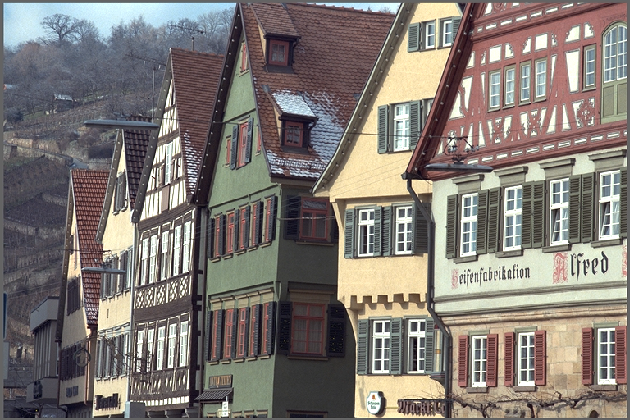
\includegraphics[width=\textwidth]{../img/liveref66.pdf}
    \legend{Fonte: \cite{livedb}}
  \end{minipage}
  \hfill
  \begin{minipage}{0.48\textwidth}
    \centering
    \caption{Imagem distorcida LIVE} \label{fig:livedist}
    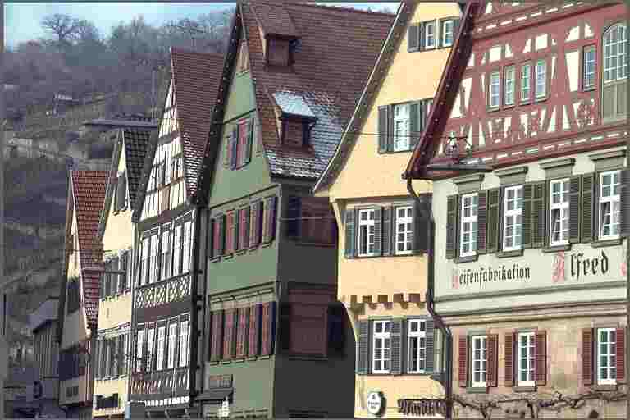
\includegraphics[width=\textwidth]{../img/liveref90.pdf}
    \legend{Fonte: \cite{livedb}}
  \end{minipage}
\end{figure}

Segundo a LIVE, o estudo que gerou as bases conduziu duas sessões de avaliação distintas. Os pesquisadores tiveram o cuidado de apresentar, em ambas as sessões, todas as imagens de referência e suas respectivas distorções. A quantidade de sujeitos no experimento foi diferente em cada sessão: na primeira, houve vinte sujeitos, na segunda, apenas treze. Os pesquisadores afirmam que a escolha das imagens para o estudo foi tal que possibilitaria uma distribuição aproximadamente uniforme das notas de avaliação, o que pode ser visualizado no histograma da \autoref{graf:liveHist}. Não foi imposta restrição de distância de visualização para a avaliação e as imagens foram mostradas aos sujeitos aleatoriamente. Para emitir suas opiniões, os sujeitos poderiam levar o tempo que necessitassem, mas só poderiam visualizar cada imagem apenas uma vez. Os pesquisadores promoveram uma pequena sessão de treinamento antes do início de cada sessão de avaliação. Estas informações e maiores detalhes podem ser obtidos no \emph{site} da referida base.

\begin{figure}[htb]
%	\label{graf:liveHist}
	\centering
	\begin{minipage}{.8\textwidth}
		\centering
		\caption{Histograma de avaliação subjetiva  --- LIVE}\label{graf:liveHist}
		\includegraphics{../../graphs/L_Hist_OSs.pdf}
		\legend{Histograma gerado a partir das opiniões dos sujeitos sobre a totalidade das imagens da base}
	\end{minipage}
\end{figure}

\begin{figure}[htb]
 \label{fig:toyaex}
 \centering
  \begin{minipage}{0.48\textwidth}
    \centering
    \caption{Imagem de referência Toyama} \label{fig:toyaref}
    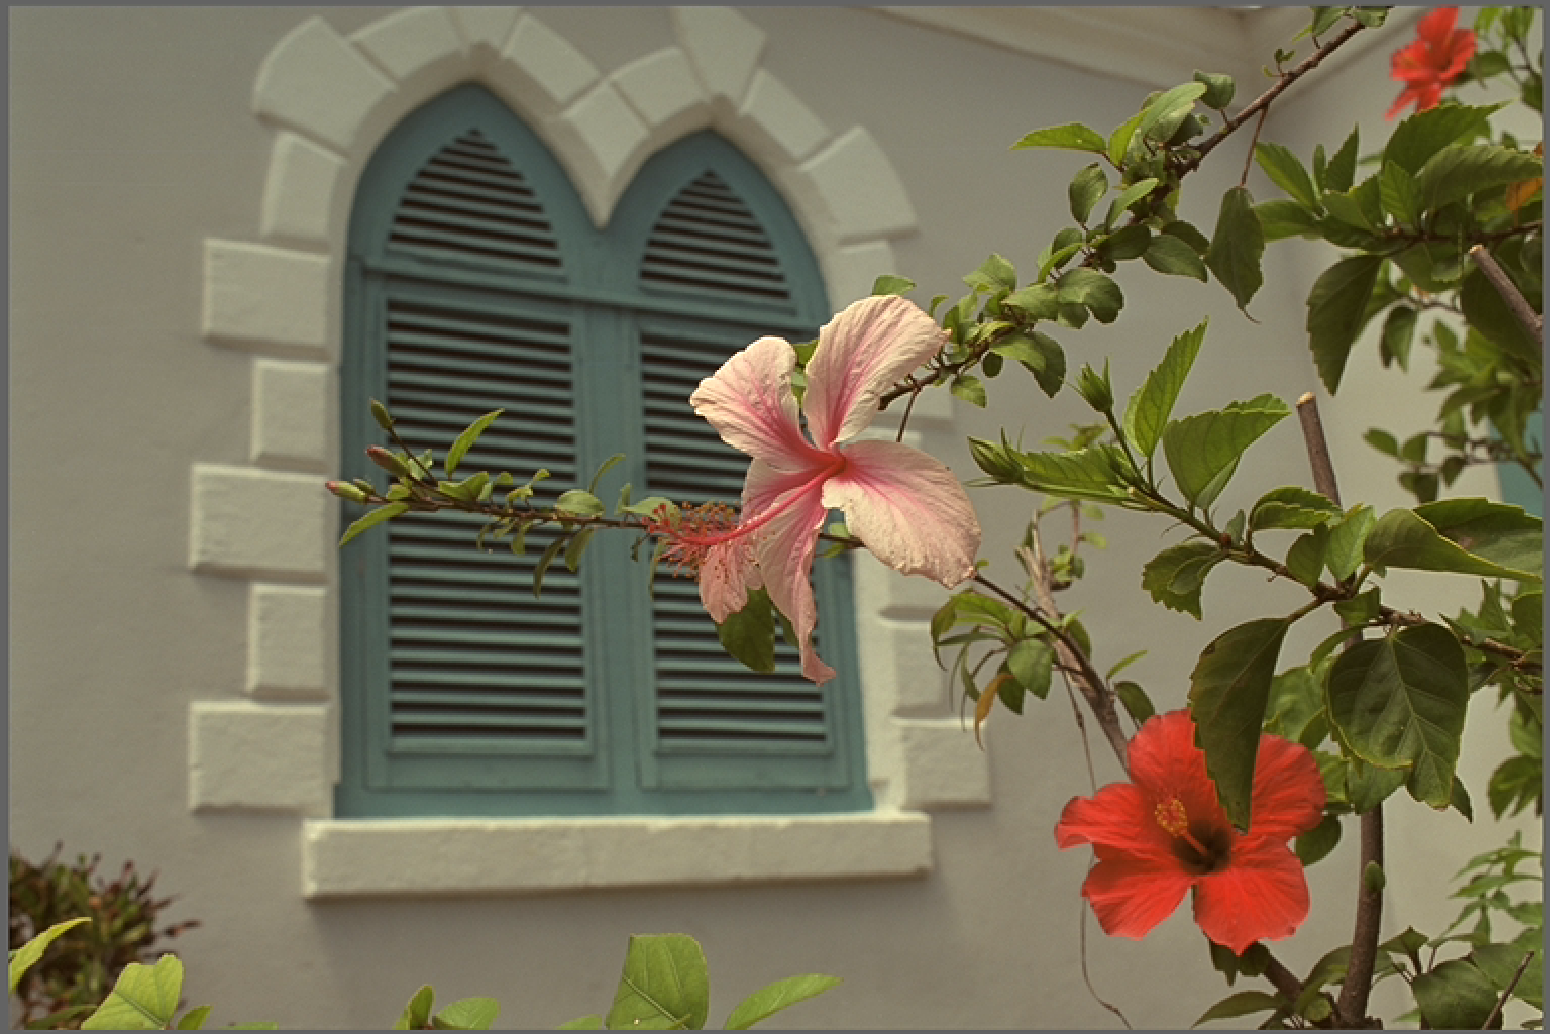
\includegraphics[width=\textwidth]{../img/toyaref07.pdf}
    \legend{Fonte: \cite{Tourancheau2008}}
  \end{minipage}
  \hfill
  \begin{minipage}{0.48\textwidth}
    \centering
    \caption{Imagem distorcida Toyama} \label{fig:toyadist}
    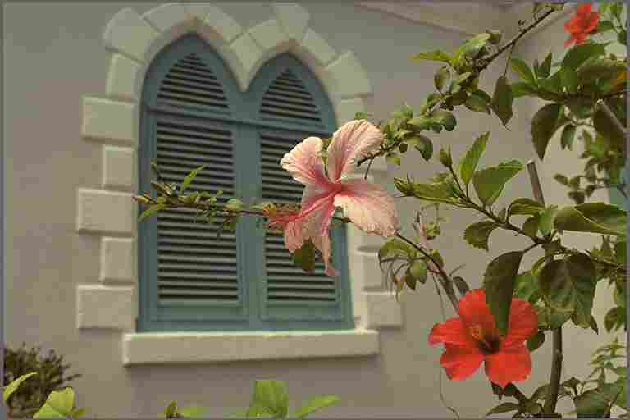
\includegraphics[width=\textwidth]{../img/toyadist07_79.pdf}
    \legend{Fonte: \cite{Tourancheau2008}}
  \end{minipage}
\end{figure}

Segundo o arquivo de informações que acompanha a base Toyama, foram dezesseis não-peritos que avaliaram as imagens dessa base, em sua maioria estudantes, não informando se houve ou não sessões distintas. Da mesma forma que a LIVE, as imagens foram apresentadas aleatoriamente, sem restrição de tempo e também com apenas uma oportunidade de avaliação para cada imagem. Neste estudo foi imposta a distância de observação igual a quatro vezes a altura da imagem. A Toyama apresenta dezesseis avaliações distintas para cada imagem, totalizando, portanto, dezesseis sujeitos no experimento. O histograma das notas de avaliação das imagens dessa base pode ser observado na \autoref{graf:toyaHist}.
 

\begin{figure}[htb]
%	\label{graf:liveHist}
	\centering
	\begin{minipage}{.8\textwidth}
		\centering
		\caption{Histograma de avaliação subjetiva --- Toyama}\label{graf:toyaHist}
		\includegraphics{../../graphs/T_Hist_OSs.pdf}
		\legend{Histograma gerado a partir das opiniões dos sujeitos sobre a totalidade das imagens da base}
	\end{minipage}
\end{figure}

Ambas os grupos de pesquisa deram a seus sujeitos uma escala com as palavras ``\emph{bad}'', ``\emph{poor}'', ``\emph{fair}'', ``\emph{good}'' e ``\emph{excellent}'', mas cada uma associou a essas palavras uma escala diferente. Além de os intervalos de avaliação serem distintos, como pode ser observado na \autoref{tab:bds}, outra diferença se faz digna de nota: a LIVE considera contínuo e linear o domínio de avaliação, enquanto a Toyama considera esse domínio discreto. Ou seja, na LIVE encontraremos notas como $4,55$, ou $9,42$ e na Toyama, apenas os inteiros entre $[1,5]$. A Toyama ainda informa que seus testes foram executados conforme as condições de avaliação apontadas no ITU-R Rec. 500-10. Veremos mais detalhes sobre essa recomendação, e outras, na sessão seguinte.

\section{Avaliação de Qualidade de Imagens}

Como dito no \autoref{chap:intro}, os atuais usos de imagens e vídeos digitais têm sua abrangência amplificada, na medida em que novos serviços surgem no mercado --- e que mais usuários utilizam esses serviços. Isso, como dito, se torna um desafio pra indústria, que precisa encontrar formas cada vez mais econômicas e eficientes de entregar seus produtos (mídias digitais) utilizando a infra-estrutura de comunicação existente e com o mínimo custo computacional e de armazenamento.

Para resolver problemas de armazenamento e tráfego, algoritmos de compressão foram desenvolvidos e são utilizados corriqueiramente. Padrões como o JPEG e MPEG são muito frequentemente utilizados por pessoas que desejam assistir vídeos online ou trasmitir fotos pelo celular. Alguns dos algoritmos utilizados hoje em dia são classificados como ``sem perdas'' (PNG e TIFF são alguns exemplos), o que significa que, uma vez descompactas, as imagens resultantes guardam as mesmas características das images originais --- o mesmo volume de dados dentro da mesma conformação espacial. Outros algoritmos, que consideram a perda de informação como razoável, são considerados ``com perdas'', e atingem taxas de compressão mais elevadas. Exemplos de algoritmos com perdas são os já citados JPG (imagem) e MPEG (vídeo).

Estabelece-se então uma relação de compromisso entre compactação (com perda de informação) e qualidade, já que é mais interessante para a indústria assumir um percentual de perda em benefício de economia de espaço e banda de tráfego. Contudo, junto com a perda de informação caminha a perda de qualidade. 

Qual o mínimo de informação para que, aferindo economia, mantenha-se a mesma qualidade percebida no produto final? Nesse contexto se situa o campo de pesquisa em qualidade de imagem. E como aferir essa qualidade? Atualmente, encontra-se duas formas distintas e dependentes: o método subjetivo de aferição de qualidade e o objetivo.

O método subjetivo ainda é o mais confiável, pois se basea na aferição a partir de observadores humanos. À pessoas são apresentadas imagens, cujas qualidades são eferidas e anotadas. Afinal, nada melhor do que o próprio cliente aferindo a qualidade do produto entregue. Essa abordagem, contudo tem algumas restrições.

A primeira grande restrição é a econômica. Para que a aferição seja feita por seres humanos é necessário que esses sujeitos sejam contratados, ou que se aloque recursos para que o material chegue até pessoas dispostas a fazer essa aferição gratuitamente. O segundo grande custo é o tempo: aferições humanas dependem de logística e tempo de processamento dos dados obtidos.

Para que se tenha uma opinião considerada estatisticamente relevante para uma população, é necessário um grande número de sessões de avaliação, com uma gama de indivíduos bastante diversa --- idealmente diversa a ponto de representar uniformemente todas as variâncias da população em questão. Essa consideração reforça as restrições de tempo e de custo financeiro. Esse tipo de avaliação é raramente executada com indivíduos ou imagens suficientes para que se possa fazer inferências a respeito do público em geral. Como dito na seção anterior (\autoref{sec:imdb}), as bases com as quais trabalhamos, largamente conhecidas e exploradas nas literaturas da área, tem poucas imagens e ainda menos avaliações. Portanto, inferências para uma população são inviáveis a partir dessas observações --- que servem apenas para fins acadêmicos.

Problemas que podem ser encontrados em estudos estatísticos são os chamados ``\emph{bias}'', que podem ser inseridos no estudo a partir da amostragem indevida da população para participação nos testes~\cite{boslaugh2008}, ainda na fase de design de tais testes. Esse tipo de consideração deve ser feita sobre as imagens que analisamos, já que estudos demonstram que ``experts'' na área de qualidade visual tentem a ser mais criteriosos em suas avaliações de qualidade; principalmente por já saberem o que procurar, no que tange erros e distribuição espacial destes. Apesar de a Toyama alegar que seus sujeitos são não-peritos, ela também alega que são estudantes de nível superior, e que, portanto, não representam bem a população de possíveis consumidores de imagens, que podem ter não só níveis diversos de educação formal como também podem ter qualquer idade.

A LIVE alega promover uma pequena sessão de treinamento antes da sessão de avaliação, mas não dá características dessas sessões. Veremos a seguir, como a forma de se colocar uma pergunta pode influenciar na resposta obtida e, portanto, questionar essa sessão prévia de treinamento é completamente válido.

Por conta dessa grande diversidade de fatores que influenciam a avaliação de qualidade de uma imagem e a validade estatística dos resultados, foram criados padrões de teste, que foram normatizados pelo ITU. Alguns exemplos são:

\begin{description}
	\item{As referências que eu tenho são todas sobre video.} Quais posso encontrar sobre imagens? Deveria consultar os padrões?
\end{description}

O método de avaliação subjetiva ainda é o \emph{benchmark} contra o qual todos os métodos objetivos são comparados. Em nosso estudo, seguindo as tendências da área, apresentamos gráficos \textbf{métrica vs. MOS}.

Por conta dessa característica humana, esse tipo de avaliação é intrinsecamente estatística, e tem sido tratada como tal. A forma desse tratamento estatístico será alvo de maiores discussões nesse trabalho.

A alternativa que surge aos métodos subjetivos é a confecção de algoritmos e estratégias computacionais que possam aferir e indicar a qualidade de uma imagem automaticamente. Claramente, uma imagem não tem para um sistema computacional o mesmo significado que tem para humanos. Nós tendemos a avaliar conteúdo e estrutura, reconhecer uma paisagem ou uma pessoa. Existem informações semânticas em imagens que fazem sentido apenas para humanos. Dessa forma, devemos buscar formas que um computador possa aferir a diferença entre duas imagens, ou buscar estrutura nelas.

As estratégias para extração de conteúdo de uma imagem podem ser distribuídas em três grupos:

\begin{description}
	\item{avaliação baseada em pixels:}
		Os métodos de extração de informação desse grupo advém principalmente de outras áreas de processamento de sinais e são razoavelmente bem conhecidas nas engenharias como um todo: MSE (\emph{Mean Square Error}, Erro Quadrático Médio) e PSNR (\emph{Peak Signal-to-Noise Ratio}, Razão de Pico Sinal-Ruído). Dentro da área de avaliação de qualidade visual, foi desenvolvida uma outra métrica em anos recentes, a MSSIM (\emph{Mean Structural Similarity Index}, Média de Índice de Similaridade Estrutural), que ganhou relevante destaque em publicações da área, apesar de sua eficiência controversa.
\end{description}
Com aferir a qualidade de uma imagem? O assunto é extenso e complexo e passa por definir o que é, de fato, qualidade. Vários fatores influenciam na avaliação da qualidade por humanos, como já dito. Uma pessoa que tenha uma conexão emocional com uma paisagem tende a atribuir maior qualidade a uma imagem que contenha a paisagem em questão. Trilhas sonoras e sincronização de áudio (especialmente no caso de fala e sincronização labial) tendem a influenciar a avaliação de qualidade de um trecho de vídeo \cite{Winkler-2005-Wiley}. Avaliações humanas são intrínsecamente estatísticas e uma boa indicação de qualidade subjetiva é a MOS (\emph{Mean Opinion Score}, inglês para ``Pontuação Média de Opinião'').

Além da avaliação humana, existem esforços para a criação de sistemas de avaliação objetiva de imagens,Existem avaliações subjetivas e objetivas. Avaliações subjetivas são feitas apresentando imagens a humanos, que as avaliam em qualidade. Muitos fatores influenciam nessa avaliação subjetiva de imagens ou vídeo, um exemplo interessante é a influência da trilha sonora na percepção de qualidade de vídeo \cite{Winkler-2005-Wiley}. Avaliações objetivas são feitas a partir de sistemas computadorizados, algoritmos criados para esse fim. Infelizmente, a avaliação objetiva ainda está muito aquém do desejado~\cite{wang-bovik2006}. , a qualidade de imagens pode ser aferida objetiva e subjetivamente. Aferições subjetivas de qualidade são feitas segundo estratégias bem definidas

O autor de \cite{Winkler-2005-Wiley} 
 % Considerações Iniciais

% Aqui é descrita toda a teoria necessária para o entendimento do trabalho. É um capítulo de caráter informativo e não deve ser grande em demasia.
% É um capítulo generalista, onde se fala sobre os principais conceitos da área
% Sub-dividido em:
%  Introdução
%  Desenvolvimento
%  Conclusão
%

% ----------------------------------------------------------
% Parte do Procedimento Experimental
% ----------------------------------------------------------
\part{Procedimento Experimental}

São três os capítulos dessa parte: Procedimento Tradicional, Procedimento por Categorias, Comparações.

\chapter{Procedimento Tradicional}

Os procedimentos de validação de uma métrica de qualidade visual passam por três testes, de acordo com as recomendações do ITU~\cite{itut2004}:

\begin{enumerate}
	\item Precisão;
	\item Monotonicidade;
	\item Consistência.
\end{enumerate}


 % Análise Comparativa

% Este é um capítudo de revisão de literatura
% Sub-dividido em:
%  Introdução: apresentada a lógica do capítulo e o que será encontrado em cada uma das seções.
%  Desenvolvimento:
%	Qual o problema analisado no trabalho?
%	Por que ele é importante?
%	O que se tem feito no mundo para resolvê-lo?
%	O ideal é se ter um estudo qeu disserte/comente os trabalhos citados, mostrando a sua relação com o problema, as vantagens e desvantagens de cada trabalho
%		citado.
%	Qual a contribuição desse trabalho? É o diferencial da proposta, principalmente, em relação às referências citadas na revisão bibliográfica.
%  Conclusão: faça referência aos pontos importantes do capítulo, que podem ser transversais às seções. Estes pontos serão, muito provavelmente, úteis ao leitor
% 		dos capítulos seguintes. Tente sempre conectar os capítulos textualmente, com 'ganchos' para o próximo assunto.
%
% Este capítulo deve omitir a teoria básica, apresentada no capítulo anterior.
% Sendo uma revisão de literatura, deve apresentar soluções dos diversos autores para o problema apresentado (ou seja, diante do problema exposto, o que tem sido feito 
% para resolvê-lo? Como? Por quem?
% Destaque como a literatura resolve o problema, vantagens e desvantagens.
%
% Este capítulo deve ser finalizado com a indicação da contribuição do trabalho e indicar o diferencial em relação as abordadas no capítulo. Maiores detalhes sobre a
% proposta do trabalho serão apresentados no próximo capítulo.

%\include{cap03} 

% Esse capítulo aborda a contribuição do trabalho. Se houver necessidade, pode-se incluir uma seção para se destacar 'uma teoria nova' (ou não citada no capítulo anterior)
% e que seja importante para o entendimento da contribuição.
%
% Sub-dividido em:
%  Introdução
%  Desenvolvimento
%  Conclusão 

% ----------------------------------------------------------
% Resultados
% ----------------------------------------------------------
\part{Resultados}

%\include{cap04}

% Aborda todos os procedimentos utilizados para a obtenção dos resultados.
% Se o trabalho for uma simulação, apresentar o cenário de simulação utilizado.
% Se for um trabalho prático, deve-se descrever o setup laboratorial juntamente com as arquiteturas eletrônicas usadas.
% A metodologia utilizada para validar os resultados/contribuições. Experiências realizadas devem ser descritas aqui.
%   Quais foram os experimentos realizados para se chegar nos resultados?
%   Como esses resultados foram validados?
% Os resultados apresentados devem ser apresentados e analisados! Analise resultados, não descreva gráficos.
% Importante é subsidiar o leitor com todas as informações usadas para a obtenção dos resultados (parâmetros devem ser especificados, quando possível, anexar as listagens
% dos resultados.
%
% Sub-dividido em:
%  Introdução
%  Desenvolvimento
%  Conclusão 
%  

% ---
% Finaliza a parte no bookmark do PDF, para que se inicie o bookmark na raiz
% ---
\bookmarksetup{startatroot}% 
% ---

% ---
% Conclusão
% ---
% \chapter*[Conclusão]{Conclusão}
% \addcontentsline{toc}{chapter}{Conclusão}
% 
% \include{concl}

% Revisão do trabalho desenvolvido
%   Objetivos do trabalho, conclusões relevantes
% Resultados / contribuições relevantes
% Resultado 1
%   Caracterização do resultado. Justificativa
%   Aspectos positivos e negativos.
% Resultado 2
% Resultado 3
% Fundamental na conclusão: TRABALHOS FUTUROS, identificar novos trabalhos que possam ser desenvolvidos sobre os resultados encontrados; fornecendo, sempre que possível, 
% 	informações e subsídios de como se pode progredir. Tente evitar esboçar uma lista de possibilidades de trabalhos futuros sem indicar como esses podem ser viabilizados
% 	a partir dos resultados encontrados.
% 
% Referências Bibliográficas: em se tratando de Ref. Bib., todas devem estar citadas no texto e listadas de acordo com a ordem de citação! Comumente adota-se o padrão de citação
% de artigos como os do IEEE

% ----------------------------------------------------------
% ELEMENTOS PÓS-TEXTUAIS
% ----------------------------------------------------------
\postextual
% ----------------------------------------------------------
% Referências bibliográficas
% ----------------------------------------------------------
\bibliography{references}

% ----------------------------------------------------------
% Glossário
% ----------------------------------------------------------
%
% Consulte o manual da classe abntex2 para orientações sobre o glossário.
%
%\glossary

% ----------------------------------------------------------
% Apêndices
% ----------------------------------------------------------

% ---
% Inicia os apêndices
% ---
%\begin{apendicesenv}

% Imprime uma página indicando o início dos apêndices
\partapendices

% ----------------------------------------------------------
\chapter{Quisque libero justo}
% ----------------------------------------------------------

\lipsum[50]

% ----------------------------------------------------------
\chapter{Nullam elementum urna vel imperdiet sodales elit ipsum pharetra ligula
ac pretium ante justo a nulla curabitur tristique arcu eu metus}
% ----------------------------------------------------------
\lipsum[55-57]

\end{apendicesenv}

% ---


% ----------------------------------------------------------
% Anexos
% ----------------------------------------------------------

% ---
% Inicia os anexos
% ---
%\begin{anexosenv}

% Imprime uma página indicando o início dos anexos
\partanexos

% ---
\chapter{Morbi ultrices rutrum lorem.}
% ---
\lipsum[30]

% ---
\chapter{Cras non urna sed feugiat cum sociis natoque penatibus et magnis dis
parturient montes nascetur ridiculus mus}
% ---

\lipsum[31]

% ---
\chapter{Fusce facilisis lacinia dui}
% ---

\lipsum[32]

\end{anexosenv}


%---------------------------------------------------------------------
% INDICE REMISSIVO
%---------------------------------------------------------------------

\printindex

\end{document}
